\documentclass[12pt, openright, oneside, a4paper, brazil]{ads-unipac-abntex2}

\usepackage{graphicx}
\graphicspath{{figuras/}{pictures/}{images/}{./}}

% Pacotes adicionais para Diagramas e Código Fonte
\usepackage{tikz}
\usetikzlibrary{shapes.geometric, arrows, positioning, shapes.symbols, fit, backgrounds}
\usepackage{listings}
\usepackage{xcolor}

% Configuração das listagens de código (Listings)
\definecolor{codegreen}{rgb}{0,0.6,0}
\definecolor{codegray}{rgb}{0.5,0.5,0.5}
\definecolor{codepurple}{rgb}{0.58,0,0.82}
\definecolor{backcolour}{rgb}{0.96,0.96,0.96}

\lstdefinestyle{tccstyle}{
    backgroundcolor=\color{backcolour},   
    commentstyle=\color{codegreen},
    keywordstyle=\color{blue}\bfseries,
    numberstyle=\tiny\color{codegray},
    stringstyle=\color{codepurple},
    basicstyle=\ttfamily\scriptsize,
    breakatwhitespace=false,         
    breaklines=true,                 
    captionpos=b,                    
    keepspaces=true,                 
    numbers=left,                    
    numbersep=5pt,                  
    showspaces=false,                
    showstringspaces=false,
    showtabs=false,                  
    tabsize=2,
    frame=single,
    rulecolor=\color{gray!30}
}
\lstset{style=tccstyle}

\newcommand{\blue}[1]{\textcolor{blue}{#1}}
\newcommand{\red}[1]{\textcolor{red}{#1}}

\autor{André Rodrigues Da Silva Junior}
\data{2026}
\orientador{Prof.Me Fabricio Araujo}
\titulo{Plataforma de Agentes de IA e Automação}
\hypersetup{pdfkeywords={agentes de IA}{GPT}{RAG}{memória}{chatbot}}

\begin{document} 
\frenchspacing 

% ----------------------------------------------------------
% ELEMENTOS PRÉ-TEXTUAIS
% ----------------------------------------------------------
\imprimircapa
\imprimirfolhaderosto

\begin{dedicatoria}
  \vspace*{\fill}
  \centering
  \noindent
  \textit{Dedico este trabalho a Deus, que me concedeu sabedoria e força. \\
  Dedico também à minha  esposa e família, pelo amor e incentivo incondicional, e aos amigos e colegas que me apoiaram ao longo desta jornada.}
  \vspace*{\fill}
\end{dedicatoria}

\begin{agradecimentos}
\noindent
Agradeço a Deus, pela orientação e pelas oportunidades concedidas. Aos meus orientadores Prof. Ricardo, Prof. Fabricio, Prof. Luiz, Prof Vitor, Prof. Igor, Prof. Cristiene, Prof. Adriana, Prof. Alan. e Prof. Daniel, pela orientação dedicada, discussões enriquecedoras e apoio em cada etapa do projeto. Agradeço aos professores do curso por todo o conhecimento compartilhado. Sou grato à minha família, especialmente aos meus pais, que sempre acreditaram em mim e ofereceram suporte emocional, sem os quais este trabalho não seria possível. Agradeço também aos colegas e amigos, especialmente os membros do grupo de estudo (Gabriel, Luiz, Luhan..), por suas sugestões valiosas e ajuda técnica. Por fim, agradeço a todos que, de alguma forma, contribuíram direta ou indiretamente para a realização deste trabalho.
\end{agradecimentos}

\begin{resumo}
Este trabalho apresenta o desenvolvimento de uma plataforma \textit{web} de agentes de Inteligência Artificial (IA) e automação. A plataforma permite criar, treinar e gerenciar agentes de conversação personalizados baseados em modelos de linguagem de grande escala (\textit{Large Language Models} - LLMs). Cada agente pode contar com memória de conversa persistente e usar técnicas de Recuperação Aumentada por Geração (\textit{Retrieval-Augmented Generation} - RAG) para incorporar informações de documentos externos.

Foram criadas funcionalidades de cadastro de agentes e edição do fluxo de conversa por meio de interface visual baseada em nós. Também houve integração com uma base de documentos usando o banco vetorial Qdrant para busca semântica. Além disso, o sistema é composto por um servidor \textit{backend} em FastAPI, um banco de dados relacional e um \textit{frontend} em Next.js.

Os resultados obtidos com os testes práticos demonstraram a viabilidade do protótipo, evidenciando que os agentes personalizados conseguiram responder de forma precisa utilizando o contexto de memória recuperado do banco de dados relacional e as fontes de informação indexadas no banco vetorial. O trabalho conclui que a integração dessas tecnologias atende aos objetivos propostos e fornece uma base funcional sólida e eficaz para automação de processos conversacionais, demonstrando alta viabilidade prática.

\noindent\textbf{Palavras-chave}: agentes de IA; modelos de linguagem; RAG; memória de conversa; vetor de documentos.
\end{resumo}

\begin{resumo}[Abstract]
This work presents the development of a web platform for Artificial Intelligence (AI) agents and automation. The platform allows the creation, training, and management of customized conversational agents based on \textit{Large Language Models} (LLMs). Each agent can maintain persistent conversation memory and use \textit{Retrieval-Augmented Generation} (RAG) techniques to incorporate information from external documents. Features such as agent registration, visual conversation flow editing, and integration with a vector document database using Qdrant for semantic search were implemented. The system consists of a FastAPI \textit{backend}, a relational database, and a Next.js \textit{frontend}. The tests demonstrated the platform's ability to create and use customized agents capable of answering questions using both conversation context and information retrieved from external documents. The project provides a functional and successful foundation for future improvements related to security, authentication, and cloud deployment.

\noindent\textbf{Keywords}: AI agents; large language models; RAG; conversation memory; vector database.
\end{resumo}

\pdfbookmark[0]{\listfigurename}{lof}
\listoffigures*
\cleardoublepage

\pdfbookmark[0]{\listtablename}{lot}
\listoftables*
\cleardoublepage

\begin{siglas}
  \item[IA] Inteligência Artificial
  \item[LLM] \textit{Large Language Model} (Modelo de Linguagem de Grande Escala)
  \item[PLN] Processamento de Linguagem Natural
  \item[RAG] \textit{Retrieval-Augmented Generation} (Geração Aumentada por Recuperação)
  \item[API] \textit{Application Programming Interface} (Interface de Programação de Aplicações)
  \item[UI] \textit{User Interface} (Interface de Usuário)
  \item[CRUD] \textit{Create, Read, Update, Delete} (Operações básicas em banco de dados: Criação, Leitura, Atualização e Exclusão)
  \item[JWT] \textit{JSON Web Token} (Token de Web estruturado em JSON)
  \item[SQL] \textit{Structured Query Language} (Linguagem de Consulta Estruturada)
  \item[ORM] \textit{Object-Relational Mapping} (Mapeamento Objeto-Relacional)
  \item[UML] \textit{Unified Modeling Language} (Linguagem de Modelagem Unificada)
  \item[UX] \textit{User Experience} (Experiência do Usuário)
  \item[OCR] \textit{Optical Character Recognition} (Reconhecimento Óptico de Caracteres)
  \item[OWASP] \textit{Open Web Application Security Project} (Projeto Aberto de Segurança em Aplicações Web)
\end{siglas}

\cleardoublepage

% ----------------------------------------------------------
% SUMÁRIO (ÍNDICE)
% ----------------------------------------------------------
\pdfbookmark[0]{\contentsname}{toc}
\tableofcontents*
\cleardoublepage

% ----------------------------------------------------------
% ELEMENTOS TEXTUAIS
% ----------------------------------------------------------
\textual

% ----------------------------------------------------------
% Introdução
% ----------------------------------------------------------
\chapter[Introdução]{Introdução}
Nos últimos anos, a Inteligência Artificial (IA) deixou de ser apenas um assunto restrito à pesquisa e passou a ocupar um espaço cada vez mais concreto no cotidiano de empresas, instituições e usuários comuns. Boa parte dessa transformação foi impulsionada pelos modelos de linguagem de grande escala, conhecidos como \textit{Large Language Models} (LLMs), como o GPT-4 (\textit{Generative Pre-trained Transformer 4}), que ampliaram de forma significativa a capacidade dos sistemas de compreender comandos em linguagem natural, responder perguntas e produzir textos com alto nível de coerência. Com isso, a interação entre pessoas e máquinas se tornou mais direta, mais acessível e, em muitos contextos, mais útil do que se imaginava há poucos anos. 

Mesmo com esse avanço, ainda existem limitações importantes. Modelos desse tipo podem gerar respostas convincentes, mas incorretas, problema frequentemente associado ao fenômeno das ``alucinações''. Além disso, quando dependem apenas do conhecimento armazenado em seus próprios parâmetros, esses sistemas enfrentam dificuldades para lidar com informações que mudam com o tempo. Em interações mais longas, outro desafio relevante é a manutenção do contexto, ya que aplicações mais complexas exigem memória persistente para que a conversa continue fazendo sentido ao longo do uso. 

É justamente nesse cenário que os agentes de IA ganham destaque. Diferentemente de assistentes conversacionais mais genéricos (comumente chamados de \textit{chatbots}), esses agentes podem ser projetados para atuar com objetivos específicos, tomar decisões orientadas por contexto, utilizar ferramentas externas e executar tarefas com um grau maior de autonomia. Na prática, isso permite desenvolver soluções mais especializadas, capazes de ir além da simples geração de texto e contribuir de forma mais efetiva para atendimento, suporte, organização de fluxos e automação de processos. 

Com base nessa perspectiva, este trabalho propõe o desenvolvimento de uma plataforma \textit{web} de agentes de IA e automação, voltada à criação, configuração e execução de agentes personalizados. A proposta busca oferecer uma solução flexível e acessível, permitindo que diferentes agentes sejam estruturados de acordo com as necessidades do usuário. Entre os objetivos específicos do projeto, destacam-se a implementação de uma interface de usuário (\textit{User Interface} - UI) intuitiva para cadastro e gerenciamento dos agentes, incluindo a construção visual de fluxos conversacionais; a integração de memória conversacional, para preservar continuidade nas interações; e a incorporação da técnica de Recuperação Aumentada por Geração (\textit{Retrieval-Augmented Generation} - RAG), que combina geração de linguagem com recuperação de informações em bases externas, ampliando a precisão, a atualização e a fundamentação das respostas produzidas pelo sistema. 

Do ponto de vista técnico, a arquitetura da aplicação será estruturada com FastAPI \cite{tiangolo2018fastapi} no \textit{backend} e Next.js \cite{verma2024nextjs} no \textit{frontend}. A escolha dessas tecnologias está alinhada à proposta do projeto, já que o FastAPI foi concebido como um \textit{framework} moderno e de alto desempenho para construção de \textit{Application Programming Interfaces} (APIs) em Python, enquanto o Next.js oferece uma base robusta para o desenvolvimento de aplicações \textit{web} \textit{full-stack} com React. Em conjunto, essas ferramentas favorecem uma organização mais clara da aplicação e criam uma base adequada para desempenho, manutenção e escalabilidade. 

A escolha desse tema surgiu da percepção de que, embora as ferramentas conversacionais baseadas em IA tenham avançado muito nos últimos anos, muitas delas ainda apresentam dificuldades quando precisam manter contexto, acessar informações externas e executar tarefas de forma realmente útil em cenários mais próximos do dia a dia. À medida que a Inteligência Artificial se torna mais presente na vida cotidiana e no ambiente organizacional, cresce também a demanda por soluções capazes de unir personalização, memória e automação em uma mesma plataforma. Ao final, espera-se obter um protótipo funcional que demonstre, na prática, como agentes de IA personalizados podem ser aplicados de maneira integrada, servindo de base para futuras pesquisas e evoluções na área de Inteligência Artificial voltada a plataformas conversacionais e automação de processos. 

 

% ----------------------------------------------------------
% Contextualização e Inovação
% ----------------------------------------------------------
\chapter[Contextualização e Inovação]{Contextualização e Inovação}
Com o avanço dos modelos de linguagem de grande escala (LLMs), a Inteligência Artificial conversacional deixou de ser apenas uma promessa tecnológica e passou a ocupar um espaço cada vez mais concreto em aplicações práticas, como assistentes virtuais, sistemas de atendimento e ferramentas baseadas em linguagem natural. Relatórios técnicos de modelos como o GPT-4 encontram justamente esse salto de capacidade, tanto na compreensão de instruções quanto na geração de respostas mais coerentes e úteis em diferentes tarefas linguísticas, o que ampliou o interesse por soluções conversacionais aplicadas a contextos reais. 

Mesmo com esse avanço, ainda existe uma diferença importante entre sistemas genéricos e agentes projetados para domínios específicos. Em cenários que exigem maior aderência ao contexto, como suporte jurídico, educacional, comercial ou corporativo, um agente configurado com objetivos claros, memória de interações e acesso a fontes relevantes tende a produzir respostas mais alinhadas ao domínio em que atua do que um modelo baseado apenas em conhecimento geral. Isso reforça a relevância de plataformas que permitam a criação de agentes personalizados, inclusive com acesso controlado a documentos privados e bases institucionais. 

A principal inovação deste trabalho está em reunir, em uma mesma plataforma, recursos que normalmente aparecem de forma separada: memória conversacional, recuperação de conhecimento por RAG \cite{lewis2020rag} e construção visual de fluxos de interação por meio do React Flow \cite{reactflow2023}. A literatura sobre agentes baseados em LLM mostra que a memória é um componente essencial para sustentar interações mais longas e contextualizadas, enquanto o RAG combina conhecimento paramétrico com recuperação em bases externas, tornando as respostas mais fundamentadas e atualizáveis \cite{santos2023rag}. Assim, o diferencial da proposta não está apenas no uso isolado dessas técnicas, mas na forma como elas são integradas em uma solução acessível, voltada à criação, configuração e execução de agentes personalizados. 

Além disso, a plataforma adota uma abordagem \textit{multi-tenant} (multilocatária) baseada no cabeçalho customizado HTTP (\textit{Hypertext Transfer Protocol}) e validação de credenciais, permitindo que cada usuário gerencie seus próprios agentes de forma separada, com maior controle sobre dados, configurações e fluxos de uso. Em arquiteturas \textit{multi-tenant}, o nível de isolamento entre locatários é uma preocupação central, especialmente quando a solução lida com dados sensíveis, documentos privados ou modelos aplicados a diferentes contextos de negócio. Nesse sentido, o isolamento entre contas não aparece apenas como uma escolha técnica, mas como um requisito importante para privacidade, segurança e organização do sistema. 

Do ponto de vista técnico, a aplicação é estruturada em uma arquitetura baseada em microsserviços integrados, o que favorece modularidade, manutenção e evolução independente dos componentes. No \textit{frontend}, o uso de Next.js \cite{verma2024nextjs} contribui para uma organização mais consistente do projeto e para a combinação entre renderização no servidor e interatividade no cliente, enquanto o Tailwind CSS facilita a criação de interfaces responsivas com base em classes utilitárias, empregando uma estratégia \textit{utility-first}. No \textit{backend}, o FastAPI \cite{tiangolo2018fastapi} oferece uma base moderna e de alto desempenho para a construção de APIs, além de favorecer integração com autenticação, gerenciamento de agentes, modelos de linguagem e repositórios vetoriais de documentos. Essa combinação tecnológica representa uma escolha atual, coerente e bem alinhada aos objetivos de engenharia de software contemporâneos \cite{sommerville2011eng}. 

Mais do que disponibilizar um \textit{chatbot}, o sistema também se propõe a apoiar a automação de tarefas. Isso significa que diferentes fluxos conversacionais podem acionar ações internas ou chamadas de API, permitindo que o agente não apenas responda ao usuário, mas também execute etapas de processo com base em regras, contexto e informações recuperadas. Em um cenário comercial, por exemplo, isso pode envolver consulta a catálogos, encaminhamento de solicitações ou apoio a rotinas operacionais. Dessa forma, a plataforma se posiciona como uma ponte entre agentes inteligentes e automação de processos, servindo tanto a demonstrações acadêmicas quanto à prototipagem de soluções aplicadas. 

\begin{figure}[ht]
\centering
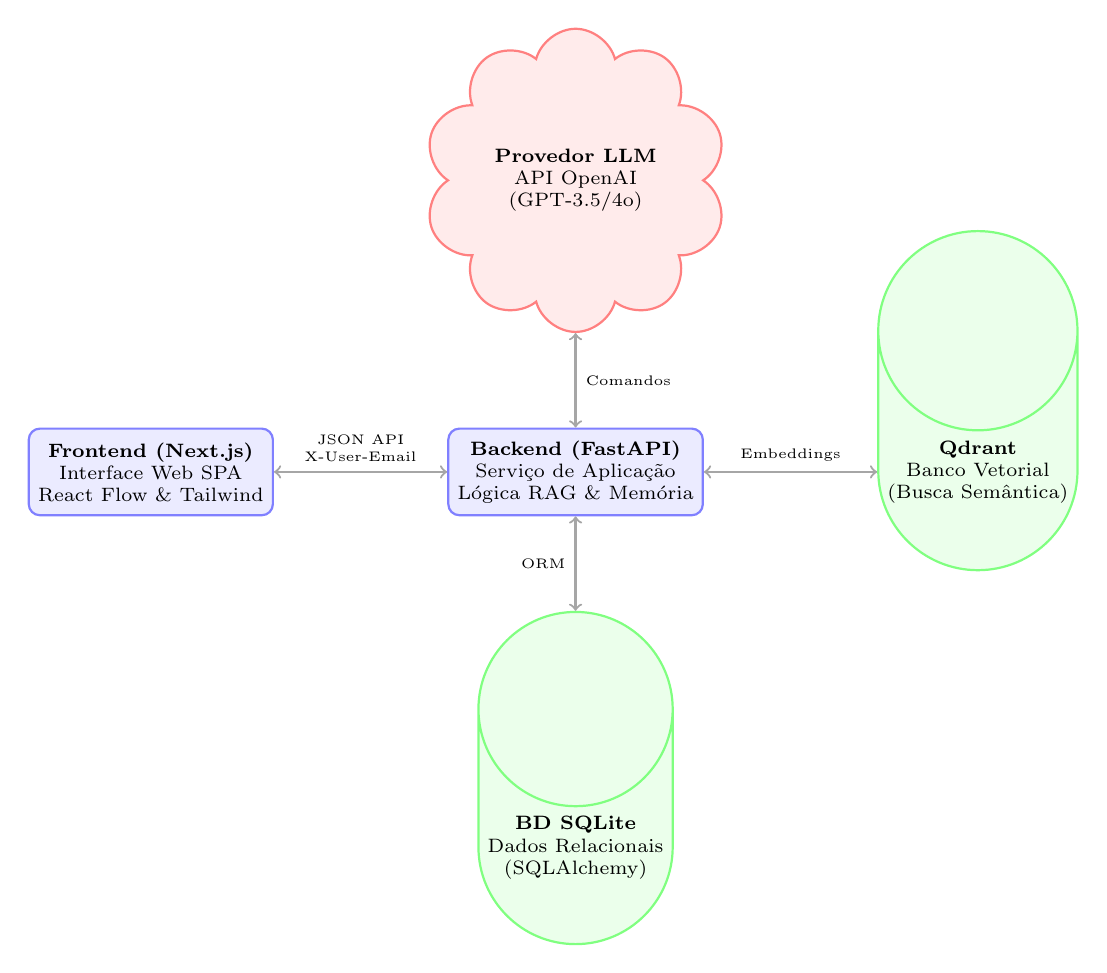
\begin{tikzpicture}[
    node distance=1.8cm and 2.2cm,
    align=center,
    box/.style={draw, rectangle, rounded corners=4pt, minimum width=2.8cm, minimum height=1.1cm, fill=blue!8, draw=blue!50, thick, font=\scriptsize},
    db/.style={draw, cylinder, shape border rotate=90, minimum width=1.6cm, minimum height=1.3cm, fill=green!8, draw=green!50, thick, font=\scriptsize},
    ext/.style={draw, cloud, minimum width=1.8cm, fill=red!8, draw=red!50, thick, font=\scriptsize},
    arrow/.style={-latex, thick, draw=gray!70}
]
    % Componentes
    \node[box] (frontend) {\textbf{Frontend (Next.js)}\\Interface Web SPA\\React Flow \& Tailwind};
    \node[box, right=of frontend] (backend) {\textbf{Backend (FastAPI)}\\Serviço de Aplicação\\Lógica RAG \& Memória};
    \node[db, below=1.2cm of backend] (sqlite) {\textbf{BD SQLite}\\Dados Relacionais\\(SQLAlchemy)};
    \node[db, right=of backend] (qdrant) {\textbf{Qdrant}\\Banco Vetorial\\(Busca Semântica)};
    \node[ext, above=1.2cm of backend] (openai) {\textbf{Provedor LLM}\\API OpenAI\\(GPT-3.5/4o)};

    % Conexões
    \draw[arrow, <->] (frontend) -- node[above, font=\tiny] {JSON API\\X-User-Email} (backend);
    \draw[arrow, <->] (backend) -- node[left, font=\tiny] {ORM} (sqlite);
    \draw[arrow, <->] (backend) -- node[above, font=\tiny] {Embeddings} (qdrant);
    \draw[arrow, <->] (backend) -- node[right, font=\tiny] {Comandos} (openai);
\end{tikzpicture}
\caption[Arquitetura Geral]{Arquitetura geral da plataforma de agentes de IA, mostrando a comunicação entre o frontend, o servidor de aplicação e a integração com o LLM e o banco de dados vetorial.}
\label{fig:arquitetura_sistema}
\end{figure}

Além de permitir a personalização, nosso sistema foca na automação de tarefas através do uso dos agentes. Diferentes fluxos de conversa podem desencadear ações internas ou chamadas de API. Por exemplo, um agente comercial pode consultar um catálogo de produtos ou encaminhar pedidos automaticamente, sempre baseando suas respostas nas informações mais recentes disponíveis (graças ao RAG). Assim, a plataforma une conceitos de agente inteligente com automação de processos, tornando-se uma ferramenta poderosa tanto para demonstrações acadêmicas quanto para protótipos de soluções de mercado.

% ----------------------------------------------------------
% Referencial Teórico
% ----------------------------------------------------------
\chapter[Referencial Teórico]{Referencial Teórico}
O avanço recente da Inteligência Artificial (IA), especialmente na área de Processamento de Linguagem Natural (PLN), está diretamente relacionado ao desenvolvimento dos Modelos de Linguagem de Grande Escala (\textit{Large Language Models} -- LLMs). Esses modelos são treinados com grandes volumes de dados textuais e conseguem compreender, interpretar e gerar textos em linguagem natural. Entre as arquiteturas que mais contribuíram para essa evolução está a arquitetura \textit{Transformer}, proposta por \citeonline{vaswani2017attention}.

A arquitetura \textit{Transformer} introduziu o mecanismo de atenção (\textit{attention mechanism}), que permite ao modelo identificar quais partes do texto são mais relevantes para compreender o contexto de uma frase ou pergunta. Diferentemente de arquiteturas anteriores baseadas em redes recorrentes, o \textit{Transformer} consegue processar informações de forma paralela, aumentando significativamente o desempenho e a eficiência em tarefas de linguagem natural. Esse avanço serviu de base para o desenvolvimento de modelos modernos como a família GPT (\textit{Generative Pre-trained Transformer}), criada pela OpenAI.

Os modelos GPT utilizam a estratégia de pré-treinamento em grandes conjuntos de textos, aprendendo padrões linguísticos, contexto e relações semânticas entre palavras. Após esse treinamento, esses modelos conseguem realizar tarefas como geração de texto, resumo, tradução e resposta a perguntas. Apesar de apresentarem desempenho elevado, os LLMs ainda possuem limitações quando precisam lidar com informações muito específicas, atualizadas ou que não faziam parte dos dados utilizados durante o treinamento do modelo.

Nesse contexto, destaca-se a técnica chamada Recuperação Aumentada por Geração (\textit{Retrieval-Augmented Generation} -- RAG), proposta originalmente por \citeonline{lewis2020rag}. Didaticamente, o funcionamento do RAG pode ser comparado a uma prova com consulta. Em sistemas convencionais sem RAG, o modelo de linguagem tenta responder às perguntas do usuário baseando-se apenas nos dados em que foi originalmente treinado (memória paramétrica). Esse cenário se assemelha a um estudante realizando uma prova sem consultar nenhum livro, o que propicia o esquecimento de detalhes ou a invenção de informações falsas. Já com o uso do RAG, o sistema realiza uma busca prévia em uma base ou biblioteca externa de documentos (memória não paramétrica), seleciona os trechos contendo a resposta exata e os anexa junto à pergunta do usuário. O modelo de linguagem então gera a resposta final baseando-se no material consultado.

Na prática, o funcionamento do RAG ocorre em duas etapas principais: primeiro, a etapa de recuperação (\textit{retrieval}), na qual o sistema realiza a busca por documentos ou trechos relevantes relacionados à pergunta do usuário; em seguida, a etapa de geração (\textit{generation}), na qual essas informações recuperadas são enviadas junto à pergunta para o modelo de linguagem gerar uma resposta mais precisa e contextualizada. Essa abordagem reduz problemas como respostas incorretas ou desatualizadas, conhecidos na literatura como alucinações de IA. Estudos recentes, como os de \citeonline{santos2023rag}, demonstram que a qualidade dos trechos recuperados influencia diretamente a qualidade final das respostas produzidas pelos modelos de linguagem.

Outro conceito importante para sistemas conversacionais modernos é a memória de conversa. Em \textit{chatbots} simples, cada mensagem pode ser tratada de maneira isolada, sem considerar interações anteriores. Entretanto, em agentes inteligentes mais avançados, torna-se necessário armazenar informações relevantes ao longo do diálogo para manter coerência e continuidade na conversa. A memória conversacional permite que o sistema relembre preferências, perguntas anteriores e informações importantes fornecidas pelo usuário durante a interação.

Segundo a literatura sobre agentes baseados em LLMs, a memória é um componente essencial para sustentar conversas mais longas e contextualizadas. Ainda assim, manter consistência em diálogos extensos continua sendo um desafio, principalmente devido às limitações de contexto dos modelos de linguagem. Por esse motivo, muitos sistemas modernos combinam memória conversacional com técnicas de recuperação de informação, como o RAG, buscando melhorar a qualidade e a continuidade das respostas geradas.

Para que a recuperação de informações funcione de forma eficiente, os documentos precisam ser convertidos em formatos adequados para busca semântica. Uma das abordagens mais utilizadas atualmente é o uso de \textit{embeddings}. \textit{Embeddings} são representações numéricas de textos em forma de vetores matemáticos capazes de preservar relações semânticas entre palavras e frases. Para um leitor não familiarizado, os \textit{embeddings} funcionam como um ``mapa semântico'' multidimensional: palavras ou conceitos com significados parecidos (como ``rei'' e ``rainha'') são convertidos em coordenadas numéricas muito próximas no espaço geométrico do mapa, enquanto termos completamente desconexos (como ``rei'' e ``computador'') ficam muito distantes entre si.

A partir dos \textit{embeddings}, torna-se possível realizar buscas por similaridade semântica, também chamadas de \textit{dense retrieval}. Diferentemente das buscas tradicionais por palavras-chave exatas (que retornam resultados apenas se houver grafia idêntica), a busca semântica considera o real significado da pergunta do usuário e do conteúdo armazenado. Dessa forma, mesmo que o usuário utilize palavras ou sinônimos diferentes daqueles presentes nos arquivos indexados, o sistema consegue compreender a intenção da busca e recuperar os trechos corretos.

No processo de indexação documental, os textos geralmente são divididos em pequenos fragmentos chamados \textit{chunks}. \textit{Chunks} são partes menores de um documento maior, criadas para facilitar a vetorização e melhorar a recuperação de informações relevantes. Como os modelos de linguagem possuem limites de processamento de texto simultâneo (a chamada janela de contexto), não é viável enviar livros ou manuais inteiros de uma só vez na requisição. A divisão em \textit{chunks} garante que apenas os parágrafos ou fragmentos contendo a resposta exata sejam extraídos e processados, otimizando o tempo de resposta e o consumo dos recursos computacionais.

Os bancos vetorial são sistemas especializados no armazenamento e gerenciamento de \textit{embeddings}. Diferentemente dos bancos de dados relacionais tradicionais, que armazenam informações organizadas em tabelas estruturadas, os bancos vetoriais são otimizados especificamente para calcular distâncias matemáticas entre vetores em alta velocidade. Entre as ferramentas utilizadas para esse tipo de aplicação destaca-se o Qdrant \cite{qdrant2020}. O Qdrant permite armazenar os \textit{embeddings} e realizar buscas semânticas eficientes, sendo amplamente utilizado em aplicações modernas de IA generativa e sistemas baseados em RAG.

No presente projeto, o Qdrant foi utilizado para armazenar os \textit{embeddings} gerados a partir dos documentos enviados pelos usuários. Assim, quando uma pergunta é realizada, o sistema busca os \textit{chunks} semanticamente mais próximos da consulta e utiliza essas informações como contexto para o modelo de linguagem gerar respostas mais precisas e contextualizadas.

Outro aspecto importante do projeto envolve a ingestão e processamento de documentos em formato PDF (\textit{Portable Document Format}). Para realizar a extração textual desses arquivos, podem ser utilizadas bibliotecas especializadas como a \textit{pypdf}. Essa biblioteca permite acessar o conteúdo textual presente na estrutura interna dos documentos digitais.

A qualidade da extração textual é fundamental para o desempenho do sistema de recuperação. Em documentos digitais, o texto geralmente pode ser extraído diretamente. Entretanto, em arquivos apenas escaneados, o conteúdo textual pode estar presente apenas como imagem. Nesses casos, torna-se necessário utilizar técnicas de OCR (\textit{Optical Character Recognition} -- Reconhecimento Óptico de Caracteres), que permitem converter imagens contendo texto em conteúdo textual processável e pesquisável de forma eletrônica.

Dessa forma, ao combinar modelos de linguagem baseados em \textit{Transformer}, memória conversacional, \textit{embeddings}, bancos vetoriais, recuperação semântica e técnicas de RAG, a plataforma desenvolvida neste trabalho busca oferecer agentes inteligentes capazes de responder perguntas de forma contextualizada, utilizando documentos externos como fonte de conhecimento e mantendo maior coerência ao longo das interações.

% ----------------------------------------------------------
% Metodologia
% ----------------------------------------------------------
\chapter[Metodologia]{Metodologia}
A metodologia adotada neste trabalho caracteriza-se como pesquisa aplicada, orientada ao desenvolvimento de um protótipo funcional de software. Esse enquadramento é coerente com a proposta do projeto, que não se limita à discussão teórica do tema, mas busca construir uma solução prática para a criação, configuração e execução de agentes de IA com memória conversacional e recuperação de conhecimento por RAG. Sob uma perspectiva de design science, o estudo também pode ser compreendido como a construção e avaliação de um artefato computacional voltado à resolução de um problema concreto, o que o aproxima de abordagens metodológicas centradas em projeto, desenvolvimento, demonstração e avaliação. 

Na etapa inicial, foi realizado o levantamento dos requisitos com base em reuniões de orientação e em revisão bibliográfica, a fim de definir as funcionalidades centrais da plataforma. A partir disso, foram delimitados os módulos responsáveis pelo gerenciamento de agentes através de operações CRUD (\textit{Create, Read, Update, Delete}), pelo armazenamento do histórico de conversas e pela integração com mecanismos de recuperação de conhecimento. Em seguida, foram elaborados o diagrama de arquitetura e o modelo de dados da aplicação, detalhando as entidades e os relacionamentos necessários ao funcionamento do sistema. A organização adotada seguiu uma arquitetura em camadas, mantendo o \textit{frontend} desacoplado del \textit{backend} por meio de APIs HTTP (\textit{Hypertext Transfer Protocol}) documentadas no ecossistema OpenAPI, o que favorece encapsulamento, manutenção e evolução mais controlada dos componentes. 

Para a interface web, adotou-se o Next.js \cite{verma2024nextjs}, framework React voltado à construção de aplicações web \textit{full-stack}, em conjunto com o Tailwind CSS, que utiliza uma abordagem \textit{utility-first} (baseada em classes utilitárias) e facilita a criação de interfaces modernas de forma mais direta. No \textit{backend}, a implementação foi realizada em Python 3.11 com o \textit{framework} FastAPI \cite{tiangolo2018fastapi}, escolhido pela boa integração com tipagem, validação de dados e geração automática de documentação interativa, inclusive com suporte a Swagger UI e ReDoc. Essa combinação tecnológica foi considerada adequada ao contexto do protótipo por favorecer produtividade, clareza estrutural e agilidade no ciclo de desenvolvimento. 

Os dados transacionais da aplicação, como usuários, agentes, sessões e mensagens, foram mantidos em um banco relacional no padrão SQL (\textit{Structured Query Language}) \cite{silberschatz2020db}, mapeados no código via ORM (\textit{Object-Relational Mapping}) SQLAlchemy. Já os documentos utilizados na etapa de recuperação foram convertidos em \textit{embeddings} e indexados no Qdrant \cite{qdrant2020}, mecanismo de busca vetorial voltado à consulta por similaridade semântica. A documentação do Qdrant destaca justamente seu uso para armazenamento e busca vetorial, com indexação em tempo real e suporte a filtros por metadados, características que o tornam apropriado para compor a etapa de recuperação em fluxos RAG. Com isso, a arquitetura separa de forma mais clara o armazenamento relacional das entidades do sistema e o armazenamento vetorial dos documentos necessários à recuperação contextual. 

O desenvolvimento ocorreu de maneira iterativa. Em um primeiro ciclo, foram implementadas as operações de cadastro, edição, listagem e remoção dos agentes, além da estrutura inicial de persistência. Em seguida, foi incorporada a funcionalidade de chat com memória de conversas, permitindo a continuidade das interações. Por fim, foi integrada a camada de RAG, conectando o modelo de linguagem à recuperação de trechos relevantes dos documentos indexados. Esse encadeamento é compatível com abordagens de design science, nas quais o artefato é refinado sucessivamente à medida que o problema é melhor compreendido e a solução é demonstrada e avaliada. 

Cada módulo foi verificado separadamente ao longo da implementação. As APIs foram inspecionadas por meio da documentação interativa gerada automaticamente pelo FastAPI e também com apoio do Postman, ferramenta usada para envio de requisições, organização de coleções e execução de testes automatizados sobre endpoints. Na interface, foram realizadas avaliações exploratórias de uso com foco na navegação, no fluxo das telas e no funcionamento das principais interações do sistema. Todo o código foi mantido em repositório Git, garantindo histórico de alterações, recuperação de versões anteriores por meio de \textit{commits} e maior rastreabilidade do processo de desenvolvimento. Em paralelo, foi produzida a documentação técnica das rotas e das estruturas de dados utilizadas na aplicação.

 

% ----------------------------------------------------------
% Desenvolvimento e Resultados
% ----------------------------------------------------------
\chapter[Desenvolvimento e Resultados]{Desenvolvimento e Resultados}
Esta seção apresenta a implementação final da plataforma e os principais resultados observados durante os testes do protótipo. A arquitetura proposta foi efetivamente traduzida para código, com um \textit{backend} desenvolvido em FastAPI responsável pelo gerenciamento das entidades da aplicação, pela persistência das conversas e pela comunicação com o modelo de linguagem, enquanto o \textit{frontend} web foi estruturado em Next.js com Tailwind CSS, oferecendo uma interface responsiva e adequada à interação com os agentes. Na camada visual, a construção dos fluxos conversacionais foi implementada com apoio do React Flow \cite{reactflow2023}, biblioteca voltada à criação de editores e diagramas baseados em nós conectados, o que permitiu representar mensagens, transições e ações de forma mais intuitiva para o usuário. 

No \textit{backend}, foram organizados módulos responsáveis pelo gerenciamento de agentes, pela base de conhecimento e pelo fluxo de conversação. A aplicação também passou a disponibilizar documentação interativa da API automaticamente no ambiente de desenvolvimento, seguindo o padrão OpenAPI adotado pelo FastAPI, com interface de exploração e teste em \verb|/docs|. Essa documentação facilitou a inspeção das rotas e tornou mais simples o processo de validação dos serviços durante o desenvolvimento. Em termos de estrutura, foram implementadas rotas para operações de cadastro, edição, listagem e remoção de agentes, além de endpoints voltados ao envio de documentos, à recuperação de contexto e à geração das respostas conversacionais. 

No fluxo de execução do chat, a mensagem enviada pelo usuário é recebida pelo servidor e combinada ao histórico da conversa e, quando aplicável, aos trechos recuperados da base documental. Esse comportamento segue a lógica dos sistemas RAG, nos quais a geração textual é apoiada por conteúdo externo recuperado por similaridade, em vez de depender exclusivamente do conhecimento paramétrico do modelo. No estágio atual do protótipo, a geração das respostas foi realizada por meio da API da OpenAI, com uso do GPT-3.5 Turbo ou GPT-4o Mini. Embora esses modelos continuem disponíveis, a documentação atual do provedor os classifica de acordo com seu custo-benefício, o que indica a possibilidade de migração para variantes mais recentes. 

Do ponto de vista dos resultados práticos, os testes funcionais mostraram que as operações centrais da aplicação estavam operando conforme o esperado. No ambiente de documentação da API e com apoio do Postman, foi possível verificar o funcionamento das rotas relacionadas aos agentes e à base de conhecimento. Já na interface web, a criação de um agente de exemplo e o envio de perguntas permitiram observar um comportamento coerente com a proposta do projeto: quando havia documentos indexados, o sistema recuperava contexto relevante antes de formular a resposta, e a saída apresentada ao usuário incluía uma seção de fontes, o que contribui para maior rastreabilidade da informação exibida. Essa lógica é compatível com o propósito do RAG de associar a resposta gerada a evidências externas. 

Além disso, o histórico das interações foi persistido no banco de dados relacional da aplicação, permitindo que mensagens anteriores fossem reutilizadas como contexto em interações posteriores. Esse aspecto é importante porque sustenta a continuidade do diálogo e aproxima o comportamento do sistema da noção de memória conversacional discutida no referencial teórico. Em conjunto com a recuperação de conhecimento, a persistência do histórico contribuiu para que o protótipo demonstrasse, na prática, a viabilidade de uma plataforma de agentes personalizados com foco em respostas contextualizadas e continuidade de uso. O código-fonte permaneceu versionado em repositório Git ao longo do desenvolvimento, o que favoreceu rastreabilidade, histórico de alterações e recuperação de estados anteriores do projeto por meio de \textit{commits}, entendidos na documentação oficial como \textit{snapshots} do histórico. 

Como limitações, o protótipo ainda depende de um mecanismo de autenticação inicial por cabeçalho simplificado de e-mail e não contempla, nesta etapa, implantação em nuvem ou endurecimento completo de segurança corporativa. Além disso, a geração das respostas depende de um serviço externo de LLM, o que implica necessidade de conectividade e custos associados ao consumo da API. Em evoluções futuras, a aplicação pode incorporar mecanismos mais robustos de autenticação e autorização, como fluxos com OAuth2 e tokens JWT (\textit{JSON Web Token}) completos, além de reforçar a proteção dos dados persistidos com práticas de armazenamento seguro e criptografia em repouso, recomendadas em guias de segurança reconhecidos como os da OWASP (\textit{Open Web Application Security Project}).

\begin{figure}[!ht]
    \centering
    \includegraphics[width=0.55\linewidth]{figuras/exemplo_dialogo.pdf}
    \caption[Fluxo de Conversa]{Exemplo de diálogo entre usuário e agente de IA: (A) pergunta do usuário, (B) contexto recuperado por RAG, (C) resposta gerada pelo modelo com citações das fontes usadas.}
    \label{fig:fluxo_conversa}
\end{figure}

O resultado prático do sistema foi verificado com várias interações de teste. No Swagger (interface de testes de rotas integrada), confirmamos o funcionamento das operações de agentes e base de conhecimento. Na interface, criamos um agente de exemplo e enviamos perguntas. Observou-se que o agente responde utilizando trechos relevantes de documentos (quando disponíveis) e inclui uma seção de ``Fontes'' nas respostas, conforme previsto. Além disso, o histórico de conversas foi registrado no banco de dados, demonstrando a memória persistente em ação. Assim, verifica-se que a arquitetura proposta atende aos objetivos estabelecidos, fornecendo respostas mais fundamentadas e contexto contínuo.

Quanto às limitações, destacamos que este protótipo não implementa autenticação OAuth2 robusta (utiliza cabeçalho customizado simplificado para desenvolvimento) nem deploy em nuvem. A integração com o LLM foi feita via serviço externo (OpenAI), implicando dependência de acesso à internet e possíveis custos de API. Embora atenda às funções principais, o sistema ainda pode evoluir em escalabilidade e segurança, por exemplo, com autenticação JWT, criptografia de dados e replicação de serviços.

% ----------------------------------------------------------
% Conclusão
% ----------------------------------------------------------
\chapter[Conclusão]{Conclusão}
Esta seção conclui o trabalho destacando as contribuições e aprendizados. Primeiro, reafirma-se que foi desenvolvida uma plataforma de agentes de IA que combina modelos de linguagem avançados com memória de conversas e técnicas de RAG, resultando em agentes personalizados. Em testes práticos, o protótipo cumpriu seus objetivos: permitiu criar agentes configuráveis, editar visualmente os fluxos de conversa e utilizar documentos externos para fundamentar as respostas geradas. Com isso, mostrou-se possível integrar recursos de memória e recuperação de conhecimento in sistemas conversacionais com LLMs.

Como principais conclusões, podemos citar:

\begin{itemize}
    \item Interface amigável: a plataforma oferece uma interface de configuração de agentes simples e intuitiva baseada em Next.js e React Flow, adequada também a usuários não especialistas. Design de UX (\textit{User Experience}) voltado à facilidade de uso torna a tecnologia complexa mais acessível.
    \item RAG com respostas fundamentadas: a incorporação de RAG garantiu que as respostas do agente fossem apoiadas em trechos relevantes de documentos. Conforme observado em estudos sobre RAG, essa abordagem diminui significativamente respostas imprecisas ou inventadas (``alucinações''), pois anexa ao resultado evidências externas.
    \item Memória conversacional contínua: a persistência do histórico de diálogo permitiu continuidade nas conversas com os agentes. Esse mecanismo de memória é justamente reconhecido na literatura como elemento-chave para manter coesão e contexto em interações de longo prazo.
\end{itemize}
Ao mesmo tempo, identificamos possibilidades de evolução do sistema. Entre elas, inclui-se a implementação de autenticação forte (por exemplo, com tokens JWT baseados em OAuth2), suporte a novos formatos de documento para consulta (como arquivos Markdown, CSV e DOCX), melhorias de escalabilidade em nuvem através de Docker/Kubernetes e o monitoramento automatizado do desempenho dos modelos (prática comum em MLOps - \textit{Machine Learning Operations}). Essas melhorias complementar foram sinalizadas durante o desenvolvimento e podem guiar trabalhos futuros.

Em suma, o protótipo desenvolvido demonstra como tecnologias emergentes de IA podem ser combinadas em uma solução poderosa e acessível. A experiência prática adquirida forma uma base sólida para pesquisas futuras em IA aplicada, indicando caminhos para avançar em sistemas conversacionais e de automação em campos como educação, saúde e atendimento ao cliente. As lições deste trabalho contribuem para a construção de sistemas de apoio automatizados mais eficientes e confiáveis.

 

% ----------------------------------------------------------
% ELEMENTOS PÓS-TEXTUAIS
% ----------------------------------------------------------
\postextual

% ----------------------------------------------------------
% Referências bibliográficas
% ----------------------------------------------------------
\bibliography{referencias}

% ----------------------------------------------------------
% Apêndices
% ----------------------------------------------------------
\begin{apendicesenv}
\partapendices

\chapter{Diagrama de Classes do Backend}
Esta seção apresenta o diagrama de classes UML simplificado do banco de dados relacional e entidades de dados modeladas através do SQLAlchemy ORM no backend Python.

As principais entidades representadas na arquitetura do banco relacional de dados da plataforma são:
\begin{itemize}
    \item \textbf{User}: Contém as credenciais básicas do usuário, permitindo o isolamento lógico das informações no ecossistema \textit{multi-tenant}.
    \item \textbf{Agent}: Representa os agentes criados na plataforma, armazenando a prompt de sistema, o modelo a ser utilizado (ex. GPT-4o Mini), configurações adicionais e o JSON do fluxo do React Flow.
    \item \textbf{AgentPermission}: Modela a possibilidade de compartilhamento de agentes entre usuários, implementando papéis como editor ou leitor.
    \item \textbf{KnowledgeBase}: Agrupador lógico de arquivos indexados e associados a um usuário dono.
    \item \textbf{KnowledgeBaseDocument}: Registra metadados e o conteúdo de texto completo extraído de cada documento enviado (como PDFs).
    \item \textbf{DocumentChunk}: Armazena os blocos de texto gerados no processo de \textit{chunking}, juntamente com o seu vetor numérico (\textit{embedding}) correspondente, permitindo o fallback de busca de cosseno local.
    \item \textbf{Conversation}: Representa uma sessão ativa de chat conectando o usuário ao agente.
    \item \textbf{ChatMessage}: Registra o histórico das mensagens (sistema, usuário, assistente) para suporte de memória de conversação.
\end{itemize}

O diagrama UML a seguir mapeia a estrutura destas entidades e os relacionamentos de chaves estrangeiras:

\begin{figure}[ht]
\centering
\begin{tikzpicture}[
    node distance=1.0cm and 2.0cm,
    classbox/.style={draw, rectangle, rounded corners=3pt, fill=gray!3, draw=black!60, thick, text width=5.5cm, font=\scriptsize},
    arrow/.style={-latex, thick, draw=black!80}
]
    % Entidades Relacionadas à Autenticação e Agentes
    \node[classbox] (user) {
        \textbf{User}\\
        \hline
        id: Integer [PK]\\
        email: String(255) [Unique]\\
        hashed\_password: String(255)\\
        provider: String(50)\\
        created\_at: DateTime
    };
    
    \node[classbox, right=of user] (agent) {
        \textbf{Agent}\\
        \hline
        id: Integer [PK]\\
        name: String(120)\\
        description: String(255)\\
        provider: String(50)\\
        model: String(120)\\
        system\_prompt: Text\\
        status: String(30)\\
        flow: JSON\\
        owner\_id: Integer [FK $\rightarrow$ User.id]
    };

    % Entidades de Conversa e Histórico (Memória)
    \node[classbox, below=1.8cm of agent] (conversation) {
        \textbf{Conversation}\\
        \hline
        id: Integer [PK]\\
        agent\_id: Integer [FK $\rightarrow$ Agent.id]\\
        title: String(255)\\
        created\_at: DateTime
    };

    \node[classbox, left=of conversation] (message) {
        \textbf{ChatMessage}\\
        \hline
        id: Integer [PK]\\
        agent\_id: Integer [FK $\rightarrow$ Agent.id]\\
        conversation\_id: Integer [FK $\rightarrow$ Conversation.id]\\
        role: String(20)\\
        content: Text\\
        created\_at: DateTime
    };

    % Relacionamento
    \draw[arrow] (user) -- node[above, font=\tiny] {1 \quad \quad \quad \quad N} (agent);
    \draw[arrow] (agent) -- node[right, font=\tiny] {1 \\ \\ N} (conversation);
    \draw[arrow] (conversation) -- node[above, font=\tiny] {1 \quad \quad \quad \quad N} (message);
    \draw[arrow] (agent.south) -- ++(0,-0.5) -| node[above, font=\tiny, near end] {N} (message.north);
\end{tikzpicture}
\caption[Diagrama UML das Entidades do Banco]{Diagrama de relacionamento UML simplificado para a persistência no banco SQLite do backend.}
\label{fig:diagrama_uml_classes}
\end{figure}

\chapter{Trechos de Código Principais}
Este apêndice inclui exemplos de código relevantes implementados na plataforma.

A Listagem~\ref{lst:crud_agent_completo} apresenta o endpoint do FastAPI para tratamento de requisições de criação de agentes:
\begin{lstlisting}[language=Python, caption={Endpoint FastAPI de criação de agentes em app/routers/agents.py.}, label=lst:crud_agent_completo]
from fastapi import APIRouter, Depends, HTTPException, status
from sqlalchemy.orm import Session
from app.database import get_db
from app import schemas, crud
from app.auth import get_current_active_user

router = APIRouter(prefix="/agents", tags=["Agents"])

@router.post("/", response_model=schemas.AgentOut)
def create_agent(
    payload: schemas.AgentCreate, 
    db: Session = Depends(get_db), 
    current_user: schemas.UserOut = Depends(get_current_active_user)
):
    existing = crud.get_agent_by_name(db, payload.name.strip(), owner_id=current_user.id)
    if existing:
        raise HTTPException(
            status_code=400,
            detail="Ja existe um agente com esse nome."
        )
    return crud.create_agent(db, payload, owner_id=current_user.id)
\end{lstlisting}

A Listagem~\ref{lst:rag_retrieval} ilustra a lógica de busca semântica no banco vetorial Qdrant, com suporte a cálculo de similaridade de cosseno local em memória como fallback:
\begin{lstlisting}[language=Python, caption={Rotina de busca semântica e similaridade em app/rag/service.py.}, label=lst:rag_retrieval]
def retrieve_context_with_sources(
    query: str,
    agent_id: int | None = None,
    kb_ids: List[int] | None = None,
    top_k: int = 4,
) -> Tuple[str, List[dict]]:
    from app.database import SessionLocal
    from app.models import Agent, DocumentChunk, KnowledgeBaseDocument
    import math

    if not query or not query.strip():
        return "", []

    with SessionLocal() as db:
        actual_kb_ids = list(kb_ids) if kb_ids is not None else []
        if agent_id is not None:
            agent = db.query(Agent).filter(Agent.id == agent_id).first()
            if agent and agent.flow:
                nodes = agent.flow.get("nodes", [])
                for node in nodes:
                    if node.get("type") == "rag" or node.get("data", {}).get("kind") == "rag":
                        kb_id_val = node.get("data", {}).get("config", {}).get("kbId")
                        if kb_id_val:
                            try:
                                actual_kb_ids.append(int(kb_id_val))
                            except ValueError:
                                pass

        if not actual_kb_ids:
            return "", []

        # Geracao de embeddings e busca
        try:
            from app.llm import embed_texts
            query_embs = embed_texts([query])
            query_vector = query_embs[0]
        except Exception:
            return "", []

        chunks_found = []
        qdrant_success = False
        try:
            from app.rag.vectorstore import search_chunks
            for kb_id in actual_kb_ids:
                hits = search_chunks(kb_id=kb_id, query_embedding=query_vector, top_k=top_k)
                for hit in hits:
                    chunks_found.append({
                        "text": hit.payload.get("text", ""),
                        "filename": hit.payload.get("title", f"KB {kb_id}"),
                        "score": hit.score
                    })
            if chunks_found:
                qdrant_success = True
        except Exception:
            pass

        # Fallback Local no Banco SQLite (Similaridade de Cosseno em Python)
        if not qdrant_success:
            db_chunks = db.query(DocumentChunk).filter(DocumentChunk.kb_id.in_(actual_kb_ids)).all()
            doc_map = {doc.id: doc.filename for doc in db.query(KnowledgeBaseDocument).filter(KnowledgeBaseDocument.kb_id.in_(actual_kb_ids)).all()}

            scored_chunks = []
            for chunk in db_chunks:
                chunk_vector = chunk.embedding
                if not chunk_vector:
                    continue
                
                dot = sum(a*b for a, b in zip(query_vector, chunk_vector))
                mag1 = math.sqrt(sum(a*a for a in query_vector))
                mag2 = math.sqrt(sum(b*b for b in chunk_vector))
                similarity = dot / (mag1 * mag2) if mag1 and mag2 else 0.0

                scored_chunks.append({
                    "text": chunk.text,
                    "filename": doc_map.get(chunk.doc_id, f"Doc #{chunk.doc_id}"),
                    "score": similarity
                })

            scored_chunks.sort(key=lambda x: x["score"], reverse=True)
            chunks_found = scored_chunks[:top_k]

        context_parts = []
        sources = []
        for i, chunk in enumerate(chunks_found):
            filename = chunk["filename"]
            text = chunk["text"]
            context_parts.append(f"--- Trecho {i+1} de {filename} ---\n{text}\n")
            sources.append({"filename": filename, "text": text[:200]})

        return "\n".join(context_parts), sources
\end{lstlisting}

\end{apendicesenv}

% ----------------------------------------------------------
% Anexos
% ----------------------------------------------------------
\begin{anexosenv}
\partanexos

\chapter{Manual de Instalação e Utilização}
Este anexo constitui o manual técnico para instalação local, configuração das variáveis de ambiente e utilização inicial do protótipo desenvolvido.

\section{Pré-requisitos do Ambiente}
Para executar a plataforma de agentes, são necessários os seguintes componentes:
\begin{itemize}
    \item \textbf{Linguagem Python}: Versão 3.10 ou superior (preferencialmente Python 3.11).
    \item \textbf{Ambiente Node.js}: Versão 18.x ou superior (para compilação do Next.js).
    \item \textbf{Docker Desktop} (Opcional): Necessário se desejar executar o banco de dados vetorial Qdrant em contêiner dedicado (caso contrário, a plataforma ativa o fallback automático no banco SQLite).
\end{itemize}

\section{Configuração do Backend (FastAPI)}
Siga os passos a seguir para o \textit{setup} do servidor de APIs no diretório \verb|/BACKEND|:

\begin{enumerate}
    \item Abra o terminal de comandos e navegue até a pasta do backend:
    \begin{verbatim}
    cd BACKEND
    \end{verbatim}
    
    \item Crie o ambiente virtual Python de desenvolvimento (\verb|venv|):
    \begin{verbatim}
    python -m venv venv
    \end{verbatim}
    
    \item Ative o ambiente virtual:
    \begin{itemize}
        \item No Windows (Powershell): \verb|.\venv\Scripts\Activate.ps1|
        \item No Windows (cmd): \verb|.\venv\Scripts\activate.bat|
        \item No Linux / macOS: \verb|source venv/bin/activate|
    \end{itemize}
    
    \item Instale os pacotes e dependências de bibliotecas descritas:
    \begin{verbatim}
    pip install -r requirements.txt
    \end{verbatim}
    
    \item Crie o arquivo de configurações de variáveis \verb|.env| a partir do modelo disponibilizado:
    \begin{verbatim}
    copy .env.exemplo .env
    \end{verbatim}
    
    \item Edite o arquivo \verb|.env| e insira suas credenciais da OpenAI API para geração das respostas e embeddings:
    \begin{verbatim}
    OPENAI_API_KEY=sua-chave-api-da-openai-aqui
    DATABASE_URL=sqlite:///./plataforma_agentes.db
    QDRANT_HOST=localhost
    QDRANT_PORT=6333
    \end{verbatim}
    
    \item Execute a inicialização do banco e migrações de dados (criação das tabelas relacionais):
    \begin{verbatim}
    python migrate.py
    \end{verbatim}
    
    \item Inicie o servidor FastAPI em modo de desenvolvimento local:
    \begin{verbatim}
    uvicorn app.main:app --reload --port 8000
    \end{verbatim}
\end{enumerate}
Com estes passos concluídos, a documentação Swagger interativa estará disponível na URL local \verb|http://localhost:8000/docs|.

\section{Configuração do Banco Vetorial (Qdrant)}
Para executar a indexação vetorial completa através do Qdrant:
\begin{enumerate}
    \item Com o Docker ativo, execute o contêiner oficial do Qdrant:
    \begin{verbatim}
    docker run -p 6333:6333 -p 6334:6334 \
      -v $(pwd)/qdrant_storage:/qdrant/storage \
      qdrant/qdrant
    \end{verbatim}
    \item Caso o Qdrant não esteja ativo na porta 6333, a aplicação backend utilizará o algoritmo nativo de busca por similaridade de cosseno (Cosine Similarity) diretamente nas tabelas de chunks do SQLite de forma automática.
\end{enumerate}

\section{Configuração do Frontend (Next.js)}
Siga os passos a seguir para o \textit{setup} e execução da interface do usuário no diretório \verb|/frontend|:

\begin{enumerate}
    \item Abra um novo terminal e navegue até a pasta do frontend:
    \begin{verbatim}
    cd frontend
    \end{verbatim}
    
    \item Crie o arquivo de variáveis de ambiente \verb|.env.local| apontando para o endpoint do backend:
    \begin{verbatim}
    NEXT_PUBLIC_API_URL=http://localhost:8000
    \end{verbatim}
    
    \item Instale as dependências JavaScript do projeto utilizando o NPM:
    \begin{verbatim}
    npm install
    \end{verbatim}
    
    \item Inicie o servidor Next.js em modo de desenvolvimento local:
    \begin{verbatim}
    npm run dev
    \end{verbatim}
\end{enumerate}
O painel administrativo do sistema poderá ser acessado pelo navegador através da URL \verb|http://localhost:3000|.

\section{Guia de Utilização do Sistema}
A navegação e testes de fluxos ocorrem da seguinte forma:
\begin{enumerate}
    \item \textbf{Acesso Inicial}: Realize o login na tela de autenticação utilizando a credencial padrão configurada para o ambiente local:
    \begin{itemize}
        \item \textbf{Usuário}: \verb|admin@plataforma.local|
        \item \textbf{Senha}: \verb|admin123|
    \end{itemize}
    
    \item \textbf{Cadastro de Agentes}: No painel, clique em ``Criar Agente''. Defina o nome, a descrição, escolha o modelo e configure a prompt de sistema que moldará a personalidade básica do agente.
    
    \item \textbf{Criação de Base de Conhecimento (RAG)}: Na guia ``Bases de Conhecimento'', crie um repositório e faça o upload de documentos PDFs de teste. O sistema extrairá o texto completo e processará a vetorização, armazenando-a.
    
    \item \textbf{Configuração Visual de Fluxos}: Utilizando o editor visual baseado em React Flow, monte a estrutura e conecte a base de conhecimento criada diretamente ao nó do agente correspondente. Salve o progresso.
    
    \item \textbf{Interação de Chat de Teste}: Abra o chat do agente recém-configurado. Envie perguntas específicas cujas respostas estejam nos documentos anexados à base de conhecimento. O sistema responderá citando os trechos e arquivos fontes nos quais se baseou, confirmando a correta integração da arquitetura RAG e a persistência do histórico na memória.
\end{enumerate}

\end{anexosenv}

\end{document}
